\section{Introduction}

The definition of a Particle System seems to depend on the application that it is being used for. It has been used to describe different techniques from modeling to rendering. 
The use of Particle Systems is a way of modeling fuzzy objects, such as water, fire, clouds, snow, smoke, etc. These don't have a smooth well-defined surface and are non-rigid objects, they are dynamic and fluid.
% quote
\begin{quote}
  ``A particle system is a collection of many many minute particles that together represent a fuzzy object. Over a period of time, particles are generated into a system, move and change from within the system, and die from the system''.
\end{quote}

Particle Systems differ in some ways from ``normal'' representations of a 3D model:
% itemize
\begin{itemize}
\item An object is not represented by a set of primitive surface elements, e.g. polygons, but as cluds of primitive particles that define its volume. 
\item A particle system is not a static entity, its particles have a cicle of life. They move and change form, new particles are created and old particles are destroyed.
\item An object represented by a particle system is not deterministic, its shar and form is not specified. Attributes are Stochastically defined, the introduction of some type of random element is used to create and change an object's shape and appearance. Attributes like a position, velocity, etc. are controlled by this random element. The element usually is controlled by some type of predefined limits.
\end{itemize}

% Head 1
\section{Particle System}

\subsection{History}
Particle systems have been in use for several decades. Since 1961 - 1962 where, perhaps, the first particle systems were implemented by three MIT students in a game called Spacewar for the PDP-1. Later in 1982, William T. Reeves, a researcher at Lucasfilm Ltd., was working on \emph{Start Trek II: The Wrath of Khan}. In the movie when a torpedo impacts with a planet a wall of fire ripples was created over the planet. Those fire  ripples were actually a lot of particle systems, or emitters, across the planet. Particle systems have been used in countless video games, animations, digital art pieces, and simulations of natural phenomena, like, fire, smoke, fog, grass, bubbles, and so on. 

% Head 2
\subsection{System}
The Particle System will have to deal with flexible quantities of elements. Sometimes zero elements, sometimes a thousand of elements. The quantity of elements is always changing because all the elements that are being generated into a system, move,change and die from the System. To compute each frame some steps must be taken into consideration: \textbf{(1)} new particles are generated into the system, \textbf{(2)} each new particle is assigned with default values, \textbf{(3)} any particles that reached the end of their lifetime will be deactivated until the emitter uses them again \textbf{(4)} the remaining particles are moved and transformed. Because of that, we're going to want to take a object-oriented approach to the implementation. Instead of defining a Particle writing only a single class, many different types of particles will have their own class extending a base particle class. We are also write a class that describes the collection of particles (the particle system itself).
Attributes of a Particle System.
\begin{itemize}
	\item Particle List
	\item Position
	\item Emission Rate
	\item Forces
	\item Current State
	\item Blending
	\item Representation
\end{itemize}

\lstset{language=C,caption={Definition of a Particle System},label=DescriptiveLabel1}
\begin{lstlisting}
abstract class ParticleSystem
{
void InitializeParticles(int index);
List<Particle> particleList;
List<int> lookUpTable;
int maxParticles;
int numParticles;
Vector3 origin;
float accumulatedTime;
Vector3 force;

public abstract Update(float elapsedTime);
public abstract Render();

public abstract void InitializeSystem();
public abstract void KillSystem();
}
\end{lstlisting}

\lstset{language=C,caption={Definition of a Particle System},label=DescriptiveLabel1}
\begin{lstlisting}
class Main
{
	ParticleSystem particleSystem;
	void Start(){
		Vector3 origin = new Vector3(0, 5, 0);
		int maxParticles = 100;
		particleSystem = new ParticleSystem(maxParticles, origin);
	}

	void Update(){
		particleSystem.Run();
	}
}
\end{lstlisting}

The objective here was to not reference a single particle in the code, yet the result screen will be full of particles. A particle system will act like an emitter, it will create and Emmit particles in a given position using a list of elements with a given size. The way the particle System handles all the particles may vary, it can use a pool of elements or simply use an array removing the last element and creating a new one in the beginning, this approaches have different impact on performance.

% Head 3
\subsubsection{Particle Generation}
Particles are generated using controlled stochastic processes. There are various processes to calculate how many particles the designer wants at any given frame in the screen. The first process controls the mean number of particles and its variance at a frame. The actual number of particles generated at a frame \emph{f} is 
\begin{equation}
\label{eqn:01}
	NParts_{f} = MeanParts_{f} + Rand() x VarParts_{f},
\end{equation}
where Rand returns a random number from -1.0 to +1.0, MeanParts\emph{f} the mean number of particles, and VarParts\emph{f} its variance.
	The Second process takes the screen size of the object as the control parameter. The mean number of particles per unit of screen area and its variance are controlled. The particle system can determine the view parameters at any given frame and calculate the screen area that it covers so a number of new particles can be set accordingly. The equation is
\begin{equation}
\label{eqn:02}
	NParts_{f} = (MeanParts_{sa}\emph{f} + Rand() x VarParts_{sa}\emph{f}) x ScreenArea,
\end{equation}
where $MeanParts_{sa}$ is the mean particles per screen area, $VarPart_{sa}$ is its variance, and ScreenArea the particle system's screen area. This method controls the level od detail of the particle system that directly affects the time required to update all the particles.

% Head 4
\subsection{Particle}

A particle system contains a collection of simple objects (\emph{Particles}). Each object in a particle system can have several attributes like:
\begin{itemize}
\item Position - The current position in world coordinates.
\item Velocity - Speed $\vec{o}^{\,s}$ and direction $\vec{o}^{\,d}$ .
\item Color - Color of the object that can change over time depending on a random element.
\item Age and Lifetime 
\item Shape
\item Size
\item Transparency
\end{itemize}
For each new individual particle generated, the system must determine default values for this, or other custom attributes.
\\ The particle starting position must me constrained to a area or a point in space. To do that a particle system has a position in three-dimensional space that defines its origin. Centered on that position the system also has a \emph{generation shape} which defines a region where all the particles will be generated. It can have a shape of a disk a square or even a spherical shape.

\lstset{language=C,caption={Definition of a Particle System},label=DescriptiveLabel1}
\begin{lstlisting}
class Particle
{
	public Vector3 Position;
	private Vector3 previousPosition;
	public Vector3 Velocity;
	public Vector3 Acceleration;
	
	public float Energy;
	public float Size;
	private float SizeDelta;
	
	public float Weight;
	private float weightDelta;
	public Color CurrentColor;
	private Color colorDelta;
}
\end{lstlisting}
Simple data structure for a Particle \emph{Csharp}.

\begin{figure}
  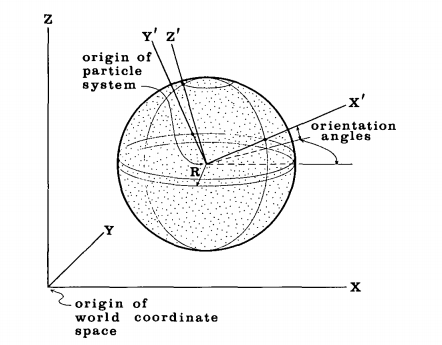
\includegraphics{particleSystem}
  \caption{Spherical Particle System.}
  \label{fig:one}
\end{figure}

	The generation shape of a particle system [\emph{figure} \ref{fig:one}] also describes the initial direction of new particles. In a spherical shape, particles will move in all directions away from the origin of the particle system. In a disk shape or a rectangular shape particles can be generated in the surface and can simply fall using gravity or have other behaviors depending on actuators like wind. The color and the shape of a particle can change using a Random element or change because of other attributes given to a certain type of particle. For example a particle can turn red depending on a heat attribute that changes over time.
	The number of possible attribute control parameters and their variants is endless. Those present here are the ones that I have found to be most useful and interesting.
 
 
% Head 5
\subsection{Particle Dynamics}
Particles within a particle system move in the three-dimensional space and can change color, shape and transparency. Particles move using its velocity vector (speed and direction), this can be affected by forces like gravity. To move a particle frame by frame we simply add its velocity vector to its position vector. This attribute changes can be controlled in global or local rate-of-change.
	There are some types of \emph{Forces} that can be applied to particles. There are Unary forces like
gravity or viscosity, N-ary forces like springs and environmental forces that can be result of collisions or repulsion. Unary forces are applied to particles independently like Gravity and Drag. Gravity is a constant acceleration in downward direction 
\begin{equation}
\label{eqn:03}
f_{gravity}(t) = \emph{m}\,\vec{g},
\end{equation}
where $\texttt{g}_{\texttt{0}} = \left [ 0\, -9.8\; \; 0 \right ]\, \frac{\emph{m}}{s^{2}}$
\\
and Drag the resistance to motion through air proportional to speed.
\begin{equation}
\label{eqn:04}
f_{drag}(t) = -k_{d}\, \Delta\, x / \Delta t = k_{d}\, \textbf{v},
\end{equation}
where $-k_{d}$ is the drag coefficient, if $-k_{d}$ = 0 then the particles are in vacuum, high values simulate drag in liquids.\\*
On the other hand N-ary forces are applied between particles.
\begin{itemize}
\item Gravitational attraction  
\item Electrical charge
\item Springs
\end{itemize}
Springs are pairs of particles connected. Two connected particles \emph{a} and \emph{b} exert force on one another proportional to the displacement of the \textbf{resting length} \emph{r} of the spring. As each spring has a rest length, if the spring length is greater than this length then the force acts to pull the two particles together, if the spring length is less than the rest length then the force acts to repel the two particles. This can be used to simulate objects with elastic properties for example cloth or ropes.
\begin{figure}
	\begin{subfigure}[b]{0.4\textwidth}
		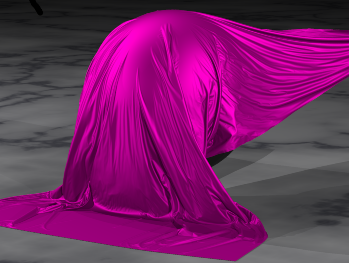
\includegraphics[width=\textwidth]{cloth1}
		\caption{Cloth simulation using a Spring system.}
		\label{fig:two}
	\end{subfigure}
	\begin{subfigure}[b]{0.4\textwidth}
		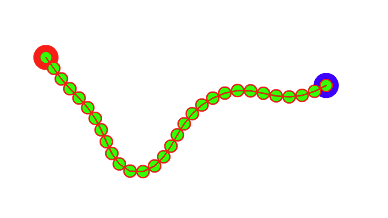
\includegraphics[width=\textwidth]{rope1}
		\caption{Rope simulation using a Spring system.}
		\label{fig:three}
	\end{subfigure}
\end{figure}
\subsubsection{Collision avoidance}
Assuming that particles don't collide with each other,as that would be too expensive to compute, for example in games that require it to run in real time considering that real time is that at least sixty frames are computed per second, so particles will only collide with the environment. For some industries the calculations per second are not important and the final result is, so there are no requirements in what takes to frames computed per second, therefore the final result will be more realistic. The basic idea here is to generate a steering force to avoid obstacles. Even if there are several obstacles in the environment, only one of them will be used at a time to calculate the avoidance force \emph{figure} \ref{fig:four}.
\begin{figure}
	\begin{subfigure}[b]{0.4\textwidth}
		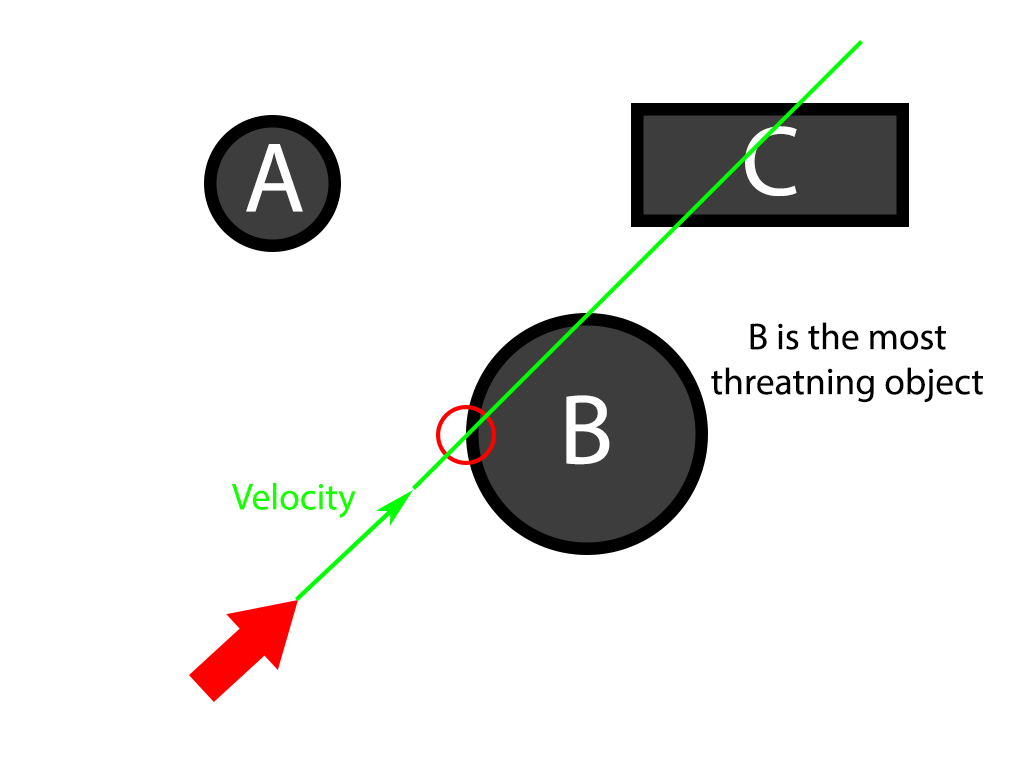
\includegraphics[width=\textwidth]{CollisionAvoidanceBasis}
		\caption{Obstacles ahead are analyzed and the closest one is selected}
		\label{fig:four}
	\end{subfigure}
	\begin{subfigure}[b]{0.4\textwidth}
		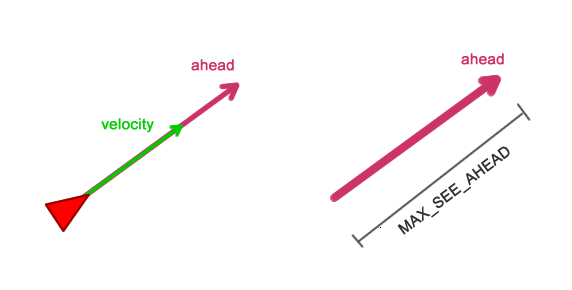
\includegraphics[width=\textwidth]{vectorahead}
		\caption{The $\vec{ahead}$ is an extension of the $\vec{forward}$}
		\label{fig:five}
	\end{subfigure}
\end{figure}
The velocity vector $\vec{\emph{v}}$ describes the direction of the element. It will be used to produce a new vector called $\vec{\emph{ahead}}$, which is a copy of the velocity vector, but with a different length \emph{figure} \ref{fig:five}.\\

This vector is calculated as follows:
\begin{equation}
\vec{\emph{S}} = P + normalize(\vec{v}) * MaxSeeAhead
\end{equation}
Where $\vec{\emph{S}}$ is the Ahead vector, $\vec{v}$ the element current velocity, normalize($\vec{v}$) takes a vector and divides all its components by its length Length = $\frac{\vec{v}}{\lVert v \rVert}$, MaxSeeAhead defines how far the particle will "see" obstacles.\\
The greater the ahead length is, the earlier the particle will compute the steering behavior to avoid the obstacle.
In order to check for collision, every obstacle must have a bounding box defined by a geometric form. Using a sphere gives the best result overall. One possible solution is to check collision using a line-sphere intersection \emph{figure} \ref{fig:four}, where the line is the ahead vector and the sphere is the obstacle. So if the distance between the center of the sphere and the ahead vector is less than the sphere radius, a collision was found.
\begin{figure}
 	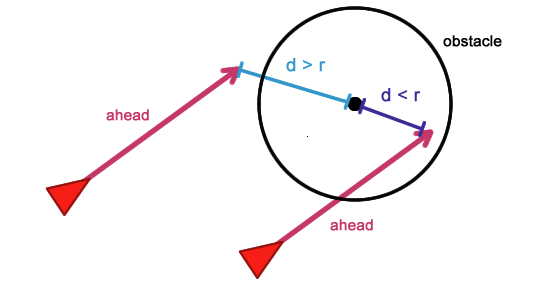
\includegraphics[scale=0.5]{collision}
 	\caption{\emph{d} is the distance and \emph{r} is the radius}
 	\label{fig:six}
\end{figure}
To determine the distance between two vectors the Euclidean distance was used. If more than on obstacle is in the way only the closest one is "threatening", selected for calculation.
\begin{figure}[H]
	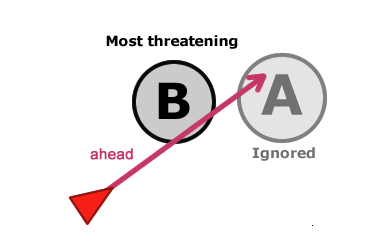
\includegraphics[scale=0.5]{Threat}
	\caption{}
	\label{fig:seven}
\end{figure}
Now we know if a certain obstacle is in the way, but, only with that information the particle would only stop or simply go through the obstacle. To make the particles avoid them, a new vector is added: the avoidance force. The avoidance force will push the particle away from the obstacle therefore avoiding it. It can be done using a the center of the sphere position and the forward vector of the particle, by subtracting them and then normalizing the result. This new vector is now added to the forward vector every frame, and that will result the particle being pushed away from the center of the object. 
% Head 6
\subsection{Particle Extinction}
Each particle has two attributes dealing with length of existence: age and lifetime. When it is generated, a particle is given a lifetime measured in frames. As each frame is computed the lifetime is decremented. A particle is deactivated or killed when its lifetime reaches zero. Age is the time that the particle has been alive (measured in frames), this value is always initialized to zero when the particle is generated. Other mechanisms, can be used for terminating a particle. If the particle ran out of bounds, these bounds can be in screen space or in projection space, and will not reenter it, then the particle can be deactivated as there is no reason to keep it alive. Other objects can be used to terminate particles, if a particle touches a certain object in the space that particle is deactivated. Using a threshold, when a particle attribute reaches a certain threshold that particle can be deactivated, for example if the color is almost red and it is a color that won't contribute to the final image that particle can be deactivated. Particles are added and removed from a collection handled by the particle system. Either we use a array or a dynamic array like a list in Csharp or an Array list in Java. Using a dynamic collection enables the option to remove and add new particles. When a particle is removed all the other ones after are shifted one index back, when one is added it goes to the end of the list.
\begin{figure}[H]
   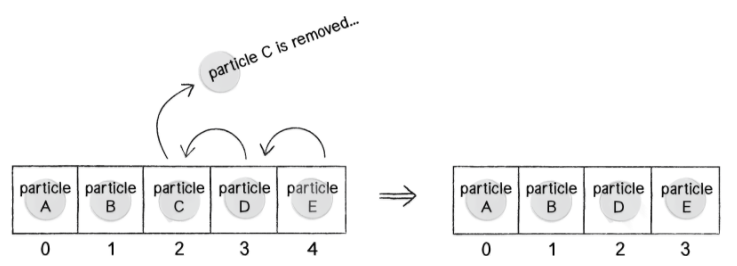
\includegraphics[scale=0.5]{arrayList}
   \caption{Removing a particle}
   \label{fig:eight}
\end{figure}
This method requires that every time a particle is removed another one must be created and initialized. Doing this for thousands of particles can be very expensive as calling the constructor method \emph{new()} every time one is added. To avoid doing this all the necessary particles are created and initialized in a collection. The objective now is, when a particle is not needed anymore it wont be removed, it will just be deactivated. But with only this, at some point all the particles would be deactivated so to fix that a Collection of \emph{int} is added. The purpose of it is to tell the particle list what is the index of next element to activate and initialize. The \emph{int} collection will act as a lookup table, when a particle is deactivated we add its index to the lookup table. When the particle system have to initialize and update new particles, it will just have to get the first index from the lookup table and use it to grab the element at that same index from the particle collection, therefore reducing the time to initialize a particle because there is no need to call the constructor and add the new particle to the list nor remove it.
\\*

\section{Conclusion}
In this project 

% Bibliography
\section{Bibliography}
\begin{itemize}
	\item[1]\url{http://www.di.ubi.pt/~agomes/tjv/teoricas/09-particles.pdf}
	\item[2]\url{http://natureofcode.com/book/chapter-4-particle-systems/}
	\item[3]\url{http://www.2ld.de/gdc2007/EverythingAboutParticleEffectsSlides.pdf}
	\item[4]\url{https://pdfs.semanticscholar.org/e791/9ff299b421d9c5ede9ee36dd87953547d557.pdf}
	\item[5]\url{http://citeseerx.ist.psu.edu/viewdoc/download?doi=10.1.1.83.6035&rep=rep1&type=pdf}
	\item[6]\url{http://www.cs.sfu.ca/~torsten/Teaching/Cmpt466/LectureNotes/PDF/10_Particle_Flocking.pdf}
	\item[7]\url{https://www.cs.drexel.edu/~david/Classes/Papers/p359-reeves.pdf}
	\item[8]\url{https://en.wikipedia.org/wiki/Particle_system}
	\item[9]\url{http://web.cs.wpi.edu/~matt/courses/cs563/talks/psys.html}
	\item[10]\url{https://www.siggraph.org/education/materials/HyperGraph/animation/particle.html}
	\item[11]\url{https://www.khanacademy.org/computing/computer-programming/programming-natural-simulations/programming-particle-systems/a/a-particle-system}
	\item[12]\url{https://www.javaworld.com/article/2071771/learn-java/simulate-fuzzy-phenomena-with-particle-systems.html}
	\item[13]\url{https://gamedevelopment.tutsplus.com/tutorials/understanding-steering-behaviors-collision-avoidance--gamedev-7777}
\end{itemize}
